% Diagram: Scheduling Considerations
% Shows prefill vs decode phases and scheduling challenges

\begin{figure}[htbp]
\centering
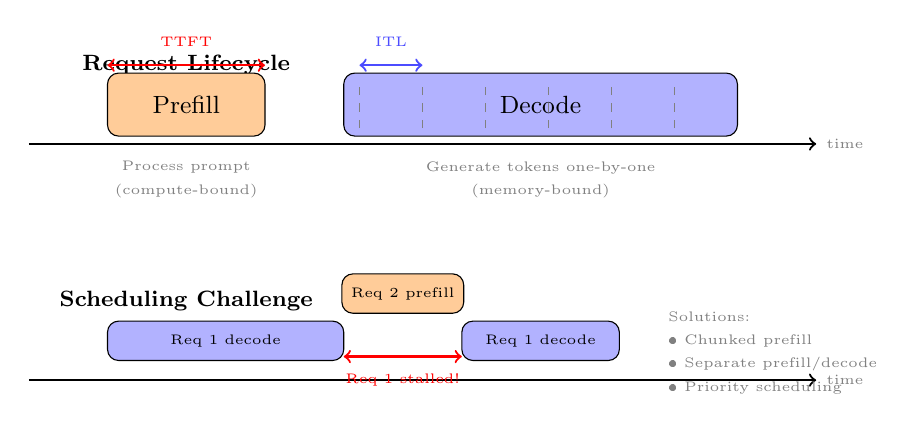
\begin{tikzpicture}[
    node distance=0.5cm,
    phase/.style={rectangle, draw, rounded corners, minimum height=0.8cm, font=\small},
    label/.style={font=\footnotesize},
    timelabel/.style={font=\tiny, text=gray}
]

% === PREFILL VS DECODE ===
\node[label] at (0, 3.5) {\textbf{Request Lifecycle}};

% Single request timeline
\draw[->, thick] (-2, 2.5) -- (8, 2.5) node[right, timelabel] {time};

% Prefill phase
\node[phase, fill=orange!40, minimum width=2cm] at (0, 3) {Prefill};
\node[timelabel] at (0, 2.2) {Process prompt};
\node[timelabel] at (0, 1.9) {(compute-bound)};

% Decode phase
\node[phase, fill=blue!30, minimum width=5cm] at (4.5, 3) {Decode};
\node[timelabel] at (4.5, 2.2) {Generate tokens one-by-one};
\node[timelabel] at (4.5, 1.9) {(memory-bound)};

% TTFT marker
\draw[<->, red, thick] (-1, 3.5) -- (1, 3.5);
\node[timelabel, red] at (0, 3.8) {TTFT};

% ITL markers
\foreach \x in {2.2, 3.0, 3.8, 4.6, 5.4, 6.2} {
    \draw[gray, dashed] (\x, 2.7) -- (\x, 3.3);
}
\draw[<->, blue!70, thick] (2.2, 3.5) -- (3.0, 3.5);
\node[timelabel, blue!70] at (2.6, 3.8) {ITL};

% === SCHEDULING CHALLENGE ===
\node[label] at (0, 0.5) {\textbf{Scheduling Challenge}};

% Multiple requests with prefill interference
\draw[->, thick] (-2, -0.5) -- (8, -0.5) node[right, timelabel] {time};

% Request 1 - already decoding
\node[phase, fill=blue!30, minimum width=3cm, minimum height=0.5cm] at (0.5, 0) {\tiny Req 1 decode};

% Request 2 - prefill arrives, blocks decode
\node[phase, fill=orange!40, minimum width=1.5cm, minimum height=0.5cm] at (2.75, 0.6) {\tiny Req 2 prefill};

% Request 1 continues but delayed
\node[phase, fill=blue!30, minimum width=2cm, minimum height=0.5cm] at (4.5, 0) {\tiny Req 1 decode};

% Stall indicator
\draw[<->, red, thick] (2, -0.2) -- (3.5, -0.2);
\node[timelabel, red] at (2.75, -0.5) {Req 1 stalled!};

% Solution annotation
\node[timelabel, anchor=west] at (6, 0.3) {Solutions:};
\node[timelabel, anchor=west, font=\tiny] at (6, 0) {• Chunked prefill};
\node[timelabel, anchor=west, font=\tiny] at (6, -0.3) {• Separate prefill/decode};
\node[timelabel, anchor=west, font=\tiny] at (6, -0.6) {• Priority scheduling};

\end{tikzpicture}
\caption{Scheduling in LLM inference. Top: A request has two phases---prefill (processing the prompt, compute-bound) and decode (generating tokens, memory-bound). Time to First Token (TTFT) measures prefill latency; Inter-Token Latency (ITL) measures decode speed. Bottom: When a new prefill arrives, it can stall in-flight decode requests, increasing their latency.}
\label{fig:scheduling}
\end{figure}
